%!TEX root = ../Thesis.tex
\chapter{Measure permeation enhancement}

\section{Studies to test peptide absorption}
The goal for an oral formulation is to achieve a high bio-availability with low a dosage variance. That is to maximize the percentage of dose absorbed, and to minimize the day-to-day variance. However in order to learn how a formulation attempt may be failing, it is needed to break down the process into individual steps. The typical three steps to consider are dissolution of the tablet, enzymatic stability and permeation enhancement. The first article included in this thesis Section \ref{article:citric}, \textit{"The role of citric acid in oral peptide and protein formulations: Relationship between calcium and proteolysis inhibition."} \cite{welling2014citric}, is a good example of the \textit{in vitro} methods used to evaluate permeation enhancement and enzymatic stability. These three steps can be understood as a chain. If just one link fails, the overall result will be poor.

Studies to test permeation enhancement ranging from early proof-of-concept development to clinical trials are listed in Figure \ref{devel_typeOf}. Beyond this list focusing on permeation studies, also dedicated studies of dissolution, peptide stability and toxicology would e.g. be required.

\begin{figure}[!htbp]
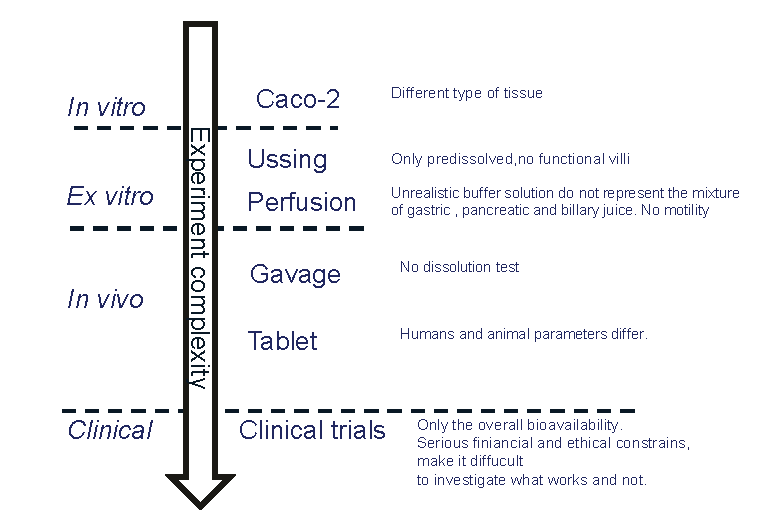
\includegraphics{graphics/typeOfExperiments.pdf}
\caption{Schematic overview of types of experiments ranging from Caco-2 to clinical. Simple experiments to not accurately simulate the actual process, and there will be a number of biases which must not be over interpreted.}
\label{devel_typeOf}
\end{figure}

In preclinical development, studies are formally categorized in latin. \textit{Ex vivo} is outside the living and \textit{in vivo}; isinside the living organism. Often \textit{in vivo} refers to animal studies only and not human studies. Studies in human are termed clinical trials. It is obviously sensible to test many new insulin analogues and formulations in fairly inexpensive and fast studies. The term \textit{in vitro}, in glass [vial], is used for lab bench studies. Lastly \textit{in silico}, in silicium, is used for computer models.
 
Medical research progress by observing relationships and propose general causal mechanisms, that are later verified and utilized. Whereas clinical trials are the most representative for the intended population of patients. One may ask why to use \textit{in vitro} studies at all, when these only are crude simulations of the clinical therapy. However, it is difficult to deduct why a clinical therapy gave no positive result, as the multiple potential steps of failure cannot be observed. Often only the final of the clinical trial can be observed. Moreover, negative confirmation is important to narrow in what part of a therapy was essential for a positive outcome. Ethical considerations limit designing clinical trials, that conflict with the best interest of patients. With \textit{in vivo} studies it is possible to test such therapies, as long as the animal suffering is kept minimal. Still, the gastro-intestinal tract is a complicated piece of machinery and it is not possible to control or measure every aspect the peptide absorption process. Both in clinical studies and \textit{in vivo} studies there can be a high subject-to-subject variance due to the variation physiology and genetic disposition. Therefore these studies may have a high unexplainable variance component. This variance component makes a step-wise incremental optimization of formulation challenging, as it becomes hard to evaluate what works, due to no significant change of bioavailability. In contrary, the lab bench \textit{in vitro} experiments offer close control of the experiment conditions. These experiments are often fast and of relatively low cost, while the reproducibility and statistical power are high. Also the \textit{in vitro} experiments can be split into individual steps as discussed in this chapter, such that every aspect increasing the bio-availability insulin can tested.

From a modeling perspective, a larger observation number is needed, especially for non-linear machine learning. Data from \textit{in vitro} is less expensive to acquire in larger numbers. The \textit{in vitro} experiments can often be crude and it is accepted as a necessary evil, that the conditions do not exactly represent completely a clinical situation. Figure \ref{devel_typeOf} lists the range of permeation experiments, and is intended to reflect this conflict between representative studies and elucidating studies.

When training machine learning models on data from \textit{in vitro} experiments, we only expect the model to reflect the experiment. The prediction of such model will only be useful to that extend the experiment is a fair generalization of the insulin absorption. With a sufficient theoretical understanding of the overall insulin absorption process and the experiment biases, we can hopefully use the model appropriately and identify the causal relationships between formulation and outcome.

\subsection{Caco-2 monolayers}
Caco-2 monolayers have been a standard screening method for intestinal drug permeability. The Caco-2 permeation model, as other permeation models, consist of a donor chamber, an epithelial barrier and a receiver chamber. Caco-2 monolayers are colonic human cancer cells, which are much more prolific and easy to handle, than primary (human non-cancer) epithelial cells. When seeded on micro porous filter (Ø 2cm) on a 12-well plate, the Caco-2 cell line will grow and form epithelial monolayers in two weeks. A typical test will use 4 mono layers per tested treatment and the study is to be repeated on a different day. A concentration of the permeation drug is applied to the donor side, and the receiver side is sampled at 4 time points to measure the diffusion rate. During the test, the nutrient rich growth media is replaced with a minimal buffer solution. The buffer solution only contain a physiological level of electrolytes such as calcium, potassium, sodium, chloride and phosphate plus an acid/base buffer. These ions maintain isotonicity and a normal electrical membrane potential. Active membrane transporter receptors in the epithelial membrane rely on a given correct membrane potential.

Within standard drug development of small molecules, a low permeability result would likely lead to discarding the given analogue, as it is easier to find a new analogue with a favorable permeability. In insulin therapy, there are few alternatives to insulin-like analogues and therefore the low permeability must be alleviated by e.g. co-formulation of permeation enhancers. To use Caco-2 monolayers to test absorption enhancers likely account for a smaller part of the use of Caco-2 monolayers. Here the permeability of insulin is already low, and may be increased by a given absorption enhancer. For surfactant enhancers at high concentration, the monolayer can be completely disrupted, while at low concentration no useful effect is observed.

\subsection{Measuring permeability}
To estimate how potent a permeation enhancer is, permeation markers have been used. An obvious marker is human insulin itself, but insulin is difficult to handle and quantification by immunobinding-assay can be expensive. A number of of alternative permeation markers are typically used to compliment insulin. One of these are $^{14}$C or $^3$H isotope labeled mannitol. Mannitol, is approximately as hydrophilic as glucose, and is thought to only diffuse passively via the paracellular pathway through the tight-junctions \cite{anderberg1992epithelial,artursson1994effect}. Unlike glucose, mannitol is not taken up by active transport, and is therefore a suitable passive transport marker. As mannitol is hydrophillic, it cannot permeate the lipophilic plasma membrane and can only permeate between the cells by the tight junctions. Mannitol is therefore a para-celullular passive permeation marker. Besides permeation of mannitol through the tight junctions, also permeation of electrolytes can be used as a marker of how open the junctions currently are.

Trans epithelial electrical resistance (TEER) can measure how open the para-cellular tight junctions are, as the junction cross sectional area is proportional to the conductivity, and conductivity is inverse resistance. TEER is an non-invasive measurement easy to apply. A certain TEER response can be translated to change of insulin permeability. E.g. lowering the epithelial resistance 50\% by the lauroyl carnitine chloride surfactant enhancer translated to a (40-fold increase) of permeability of insulin in Caco-2 model \cite{welling2014citric}.

FITC-dextran 4000 dalton (FD4) is a florescent labeled sugar polymer of similar hydrophilicity and size as insulin. FD4 can mimic insulin as transport marker as it has similar molecular weight and hydrophobicity \cite{vernon1999insulin}. FD4 on the other hand has no enzymatic instability and can be used to estimate what would have been the permeation of unchanged insulin, disregarding the enzymatic cleavage in the luminal space. FD4 can be specifically and accurately quantified, as it is a strong fluorophore.



\subsection{Calculating permeability}
\label{calcPerm}
Gradient driven diffusion of mannitol, FD-4 and insulin across the epithelial barrier are first order processes, where the transport per time (aka. flux) is proportional to the concentration gradient $C_i$ ($mol/L$). Only a few percent of the total amount of transport marker will permeate the barrier and therefore will $C_i$ be approximately unchanged throughout the experiment. Hereby becomes the apparent permeability $\bm{P}_{app}$ proportional to the transport rate or flux $\bm{J}$ ($mol/s$), which is usually estimated by sampling the receiver basolateral side 4 times. When plotting receiver concentration versus time, a fitted ordinary least squares slope is used as the overall flux through out the experiment. Permeability is the flux, per concentration gradient and corrected for the cross sectional area of the chamber, $\bm{A}$ ($cm^2$). Therefore the apparent permeability is calculated as

$\bm{P}_{app} = \bm{J} / \bm{A} / \bm{C}_i = \frac{d\bm{C}_r}{dt} / \bm{A} / \bm{C}_i \quad ,$

where $\frac{d\bm{C}_r}{dt}$ is the slope of ordinary least squares regression of receiver chamber concentration versus time. The intercept with x-axis (time) is interpreted as the lag time, which is the time it takes to saturate the mucus layer, the thin unstirred water layer and the epithelial junctions. The lag time is typically a couple of minutes depending whether using Caco-2 or Ussing chamber. To observe an apparent constant flux e.g. throughout a one hour experiment is normal. The small decrease in concentration gradient of some few percent throughout the study may ideally have caused deceleration of the flux. However, it is possible that the actual permeability of the epithelial barrier is increasing through the one hour flux study due to slow deterioration by the absorption enhancer, and therefore a constant flux is observed. In control epithelial barriers without absorption enhancer treatment, the barrier integrity is not expected to decline, but at the same time the flux is very low, so the concentration gradient do not change.

\begin{figure}[!htpb]
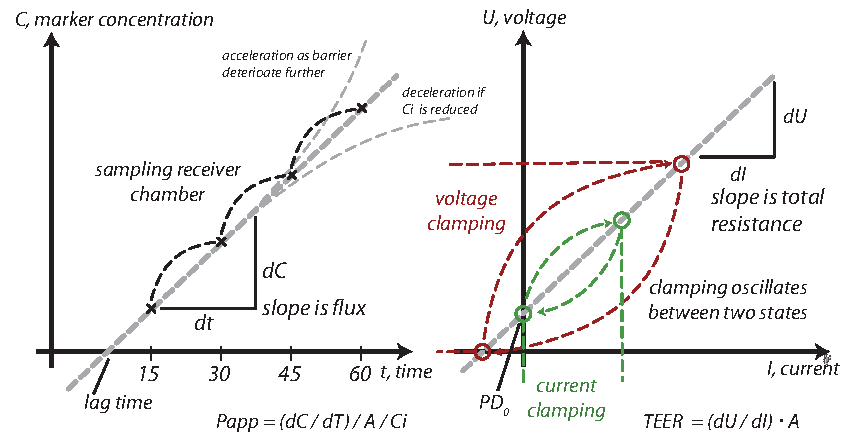
\includegraphics[width=\textwidth,height=\textheight,keepaspectratio]{graphics/samplingClamping.pdf}
\caption{Illustration of how \textit{(left)} $\bm{P}_{app}$ and \textit{(right)} TEER is calculated.}
\label{meassure_TEERPapp}
\end{figure}

The tight junctions are ideally water filled channels between the cells of the barrier. The water in the channels can be thought to have specific conductance depending on the concentration and diffusability of ions. When tight junction are widened, the cross-sectional area of tight-junction is changed. Similarly as marker flux is driven by a concentration difference, the electrical current $\bm{I}$ (Ampere $\mu A$) is driven by an electrical potential difference $\bm{U}$ (Voltage $V$). The electrical current $\bm{I}$ is analogue to the flux $\bm{J}$ and potential difference $\bm{U}$ to $\bm{C_i}$. Therefore the membrane conductivity corrected for membrane area $\bm{G_A}$ area can be expressed in parallel to $\bm{P_{app}}$, such that

$\bm{G_A} = \bm{I} / \bm{A} / \bm{U} \quad .$

The inverse of $\bm{G_A}$ is named TEER (trans epithelial electrical resistance)(Ohm cm$^2$) in drug transport studies. To summarize both $\bm{P_{app}}$ and inverse TEER describe how readily a flux of either molecules or ions are driven through the epithelial barrier by respectively a concentration gradient or a electrical potential gradient. 

Figure \ref{meassure_TEERPapp} describes how to calculate the slopes for $P_{app}$ and TEER. For $P_{app}$  the receiver concentration $\bm{C}_r$ is plotted as a function of time, the slope represents flux $\bm{J}$. TEER is either measured with voltage or current clamping. To measure TEER with voltage clamping is to control the electrical gradient (potential difference) with electrodes and measure the actual current. Whereas, current clamping is to drive a specified flux of ions (current) through the epithelial barrier and record the electrical gradient. In either case is the membrane potential difference $U$ plotted as a function of current. The slope represents TEER not corrected for area. At zero applied current, the potential difference is not neccesarily zero, as the epithelia has an active energy dependent ion transport. The slopes obtained by current clamping and voltage clamping are exactly the same.

For direct measurement of the intrinsic permeability of a given drug molecule without permeation enhancers, TEER is mainly used to check barrier integrity. For measuring the potency of permeation enhancers to increase permeability, TEER can be used as indicator hereof. To directly measure the permeation of insulin would be preferable, but this is more slow, expensive and unlikely to in already published results. As the current and potential difference can be manipulated with electrodes, the time resolution for TEER measurements is ideally in seconds. The time resolution for permeation markers is limited by the sampling rate and accuracy of the concentration determination. However, in Caco-2 studies the sampling rate for both TEER and $\bm{P}_{app}$, the sampling rate of Caco-2 studies are typically once per 15 minutes.

As the potency of permeation enhancers can vary greatly, it is not meaningful to test all enhancers by the same concentration. Like a under- and over-exposure in photography, a too low concentration will have no measurable effect and a too high concentration will kill the epithelial cells. The \%TEER-decrease describes how much resistance the epithelium looses by a given permeation enhancer at one specific concentration. The measured \%TEER decrease is likely a sigmoidal curve as a function of the logarithmic enhancer concentration. Whitehead \textit{et al} produced the data set, that the permeation model of this thesis has been based on. Every enhancer was tested at 1\%, 0.1\% and 0.01\% (w/w) and the resulting \%TEER decrease was measured \cite{whitehead2008safe}. If a given enhancer had no effect the total TEER would not change. In opposite, if the enhancer was overdosed, the epithelium would practically be dissolved and TEER would plummet to zero. In order to summarize how a permeation enhancer performed across the three concentrations, I decided to simply compute the average \%TEER decrease for the three concentration levels. This potency average was named Tpot. If Tpot=0.5, the enhancer likely elicited ratio-TEER decreases (0.90, 0.50, 0.10) at the respective concentrations. Likewise for Tpot=.9 the ratio-TEER decreases may have been (1.00,0.95,0.75). To predict the \%TEER-decrease at one specific concentration is both not that useful and may be difficult. To predict the potency of a permeation enhancer as defined by Tpot is more useful and realistic. If the potency of one enhancer is mediocre, it may be acceptable if the predicted solubility is outstanding. Then a high concentration of the permeation enhancer can be released at once.

\section{Mechanisms of absorption enhancement in oral formulations}
The formulation part of oral peptide therapy is mainly to ferry the highest possible total and relatively amounts of insulin unchanged through the upper gastro-intestinal tract. The two major barriers are enzymatic degradation and poor epithelial permeability. Other barriers are the mucus and thin unstirred water layer on top of the epithelia. These barriers are not regarded as prominently rate limiting bottle necks and are not given as much attention.(cite)

\subsection{Preventing and measuring enzymatic degradation}
Enzymatic stability of peptides vary greatly in the intestinal tract. The time span insulin can remain unchanged after tablet dissolution in the small intestinal lumen is considered to be from a single minutes up to 15 minutes \cite{welling2014citric}. Enzymatic degradation rate ($V_i$) is assumed to follow Michalis-Menten kinetics, which describes the degradation rate per enzyme as a function of substrate/peptide concentration $[S]$, enzyme-substrate binding constant ($K_m$), and max enzyme degradation speed $V_{max}$.

$V_i = \frac{V_{max} [S]}{K_{M}+[S]}$

The Michales-Menten kinetics describe, that at very low concentrations of substrate (peptide), the degradation rate will be proportional to the concentration of insulin in the luminal space, thus a first order decay process. 
The Michaelis-Menten kinetics opens for three ways to limit relative peptide degradation. First the apparent $K_m$ binding constant can be increased by adding a competitive substrate. The enzyme will then bind to another substrate such as soy bean peptides or Bowman-Birk compounds. A very potent non competitive inhibitor would bind strongly to the enzyme, such that only a small amount of inhibitor would be needed. Such non-peptide inhibitors are in practice toxic and not suited for chronic treatment \cite{bernkop1998use,murthy1980effect}. 

A second option, which is used in the article \cite{welling2014citric} of this thesis, is to lower the apparent $V_{max}$. Citric acid itself is not a substrate of trypsin or chymotrypsin. As citric acid is dissolved, it will partly release protons into the luminal space and thereby lower pH. The enzymes trypsin and chymotrypsin have a 10-fold lower $V_{max}$ at pH=4.
The last way to inhibit the relative degradation is to release as much substrate as fast as possible into the luminal space. As the substrate concentration increase $[S] >> K_m$ and $V_i \approx V_{max}$ there will be a theoretical upper limit for how much insulin can be degraded per time. Driving up the concentration of insulin, will surpass the linear range of degradation and approach the $V_{max}$. This approach could fairly be called hit and run, as enough insulin is released in such a short time and location, that the enzyme cannot degrade all at once. The latter approach is highly dependent on the dissolution time of the tablet. If the tablet dissolves over an hour, the insulin would be released very slowly in small concentrations, and the enzymes would have plenty of opportunity to degrade all insulin. To simply drive up the insulin content of the tablet is not a likely successful strategy, as the insulin is very costly to produce. Also, there can be an upper boundary of how much insulin, that can be included in one tablet due to drug safety. Otherwise a case of unexpected high bioavailability could lead to a hazardous overdose and acute hypoglychemia.

\subsection{Article: \textit{The role of citric acid in oral peptide and protein formulations: Relationship between calcium and proteolysis inhibition}}
\label{article:citric}
\newpage
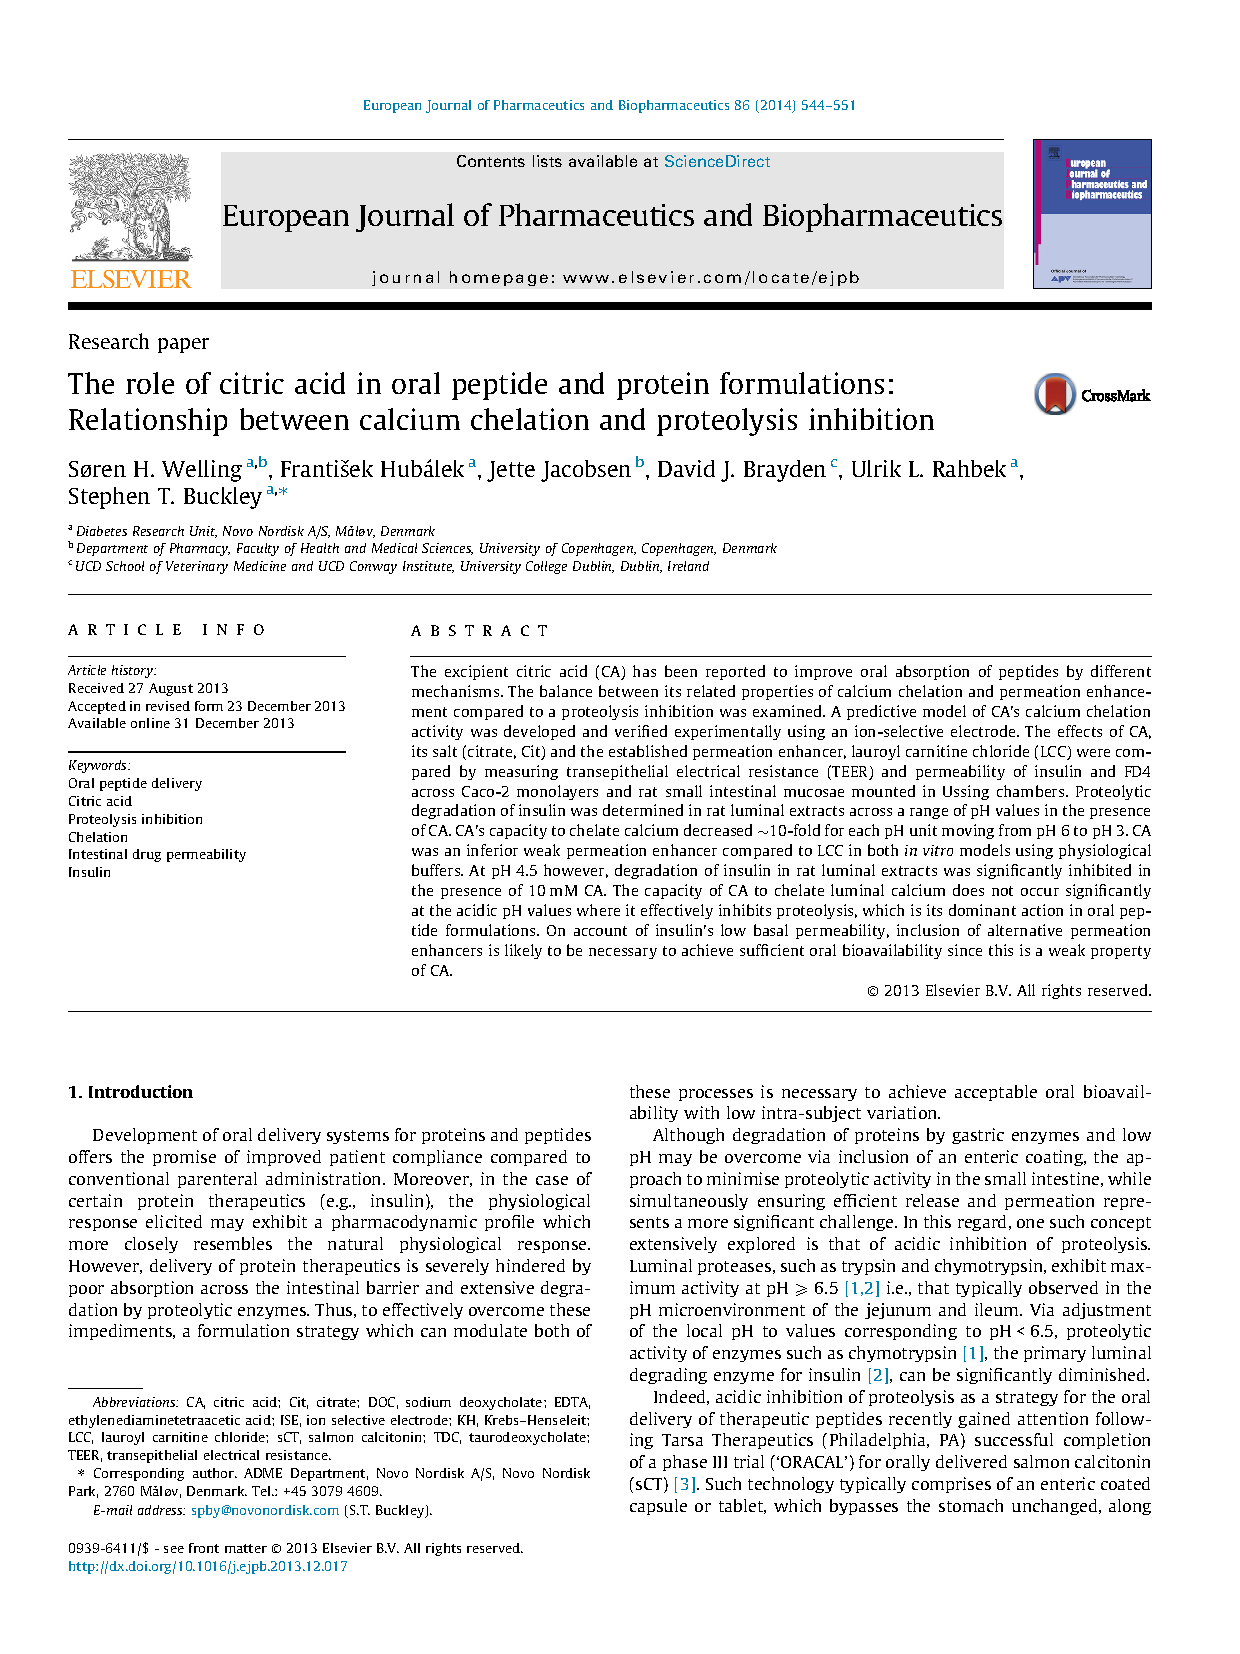
\includepdf[pages={1-},scale=0.90,pagecommand={\pagestyle{myruled}}]{chapters/citricAcid.pdf}